\documentclass[xetex,table]{beamer}

\usepackage[autostyle]{csquotes}
\usepackage{hyperref}
\usepackage{color}
\usepackage{setspace}
\usepackage{listings}
\usepackage{minted}

\usetheme{metropolis}

\usemintedstyle{perldoc}
\definecolor{codebackground}{rgb}{0.96,0.96,0.75}

\title{ARM64 + FPGA and more:\\Linux on the Xilinx ZynqMP}
\subtitle{Opportunities and challenges from a powerful and complex chip}
\author{Luca Ceresoli, AIM Sportline\\
  \href{mailto:luca@lucaceresoli.net}{\tt luca@lucaceresoli.net}\\
  \url{http://lucaceresoli.net}
}
\date{FOSDEM 2018}

\begin{document}

\maketitle

\begin{frame}{About me}
  \begin{columns}
    \column{0.4\textwidth}
    \includegraphics[width=\textwidth]{images/aim-products.jpg}

    \column{0.6\textwidth}
    \begin{itemize}
    \item Embedded Linux engineer\\
      at AIM Sportline\\
      {\footnotesize\url{http://www.aim-sportline.com/}}
      \begin{itemize}
      \item Develop real products on custom hardware
      \item Kernel, bootloader, drivers
      \item Integration, build system
      \end{itemize}
    \item Open source enthusiast
      \begin{itemize}
      \item Contributor to Buildroot and a few other projects
      \end{itemize}
    \end{itemize}
  \end{columns}
\end{frame}

\section{Hardware overview}

\begin{frame}{Block diagram (simplified)}
  \begin{center}
    \includegraphics[height=0.9\textheight]{images/block-diagram.pdf}
  \end{center}
\end{frame}

\section{Development tools}

\begin{frame}[standout]
  FPGA development
\end{frame}

\begin{frame}{FPGA Development Tools --- Xilinx}
  Xilinx Vivado Design Suite
  \begin{itemize}
  \item Vivado: design FPGA to bitstream
  \item XSDK: eclipse IDE for firmware development
  \item Runs on Linux
  \item Has a zero-cost version (has most features, not the advanced
    ones)
  \item Closed source, huge, has some bugs and issues
  \end{itemize}
\end{frame}

\begin{frame}{FPGA Development Tools --- Open source}
  \begin{itemize}
  \item No open source FPGA toolchain available
  \item Bitstream reverse engineering in progress
    (\url{https://symbiflow.github.io/})
  \end{itemize}
\end{frame}

\begin{frame}[standout]
  BSP components
\end{frame}

\begin{frame}{U-Boot}
  \begin{itemize}
  \item Xilinx is active in mainlining
  \item Discussion: \texttt{U-Boot@lists.denx.de}
  \item Mainline U-Boot enough to boot
  \item Newer boards are available at
    \url{https://github.com/xilinx/u-boot-xlnx}
  \item Note: ZynqMP cannot boot U-Boot the ``normal'' way, see {\em
    Booting} section later
  \end{itemize}
\end{frame}

\begin{frame}{Linux kernel}
  \begin{itemize}
  \item Xilinx is active in mainlining
  \item Discussion: \texttt{linux-arm-kernel@lists.infradead.org}
  \item Mainline Linux: partially implemented
  \item Development in progress at
    \url{https://github.com/xilinx/linux-xlnx}\\
    (especially the \texttt{master} branch)
    \begin{itemize}
      \item ``Hard'' silicon features
      \item Recent UltraScale+ IPs from Xilinx, mostly video-related
    \end{itemize}
  \end{itemize}
\end{frame}

\begin{frame}[standout]
  Build system
\end{frame}

\begin{frame}{Available workflows}
  Typical ways to build the software stack for Xilinx products:
  \begin{itemize}
  \item The {\bf ``Xilinx workflow''}
    \begin{itemize}
    \item Officially supported by Xilinx
    \end{itemize}
  \item The {\bf ``Community workflow''}
    \begin{itemize}
    \item Similar to other open source projects
    \item Supported by the community (with Xilinx contributions)
    \end{itemize}
  \item Other/mixed workflows
  \end{itemize}
\end{frame}

\begin{frame}{The Xilinx workflow}
  \begin{itemize}
  \item FPGA: Vivado
  \item Baremetal and bootloaders: XSDK
  \item Petalinux
    \begin{itemize}
    \item A Xilinx-specific embedded build system
    \item Nowadays internally uses Yocto
    \end{itemize}
  \item Yocto layers on \url{https://github.com/xilinx}
    \begin{itemize}
    \item A {\tt meta-xilinx-bsp} fork
    \item {\tt meta-xilinx-tools} to use Xilinx tools during the build
    \item {\tt meta-petalinux}: a distro layer
    \item Note: these layers will soon be moved to subdirs of {\tt
      meta-xilinx}
  \end{itemize}
  \end{itemize}
\end{frame}

\begin{frame}{The Community workflow}
  \begin{itemize}
  \item FPGA: Vivado
  \item A little bit of XSDK
  \item Yocto {\tt meta-xilinx-bsp} layer\\
    {\footnotesize\url{https://git.yoctoproject.org/cgit/cgit.cgi/meta-xilinx/}}
    subdir {\tt meta-xilinx-bsp}
    \begin{itemize}
      \item Until a few weeks ago: in the top dir, and called {\tt meta-xilinx}
  \end{itemize}
  \item Goal: follow the common practices in FOSS/Yocto
  \item Not all features supported
  \end{itemize}
\end{frame}

\begin{frame}{Other resources}
  \begin{itemize}
  \item meta-xilinx mailing list
    \begin{itemize}
    \item {\footnotesize\url{https://lists.yoctoproject.org/listinfo/meta-xilinx}}
    \item Discussion on the Yocto layers
    \item Also for general discussion about Linux on Xilinx
      hardware
    \end{itemize}
  \item {\small\url{https://github.com/topic-embedded-products/meta-topic}}
    \begin{itemize}
    \item Support for boards by Topic Embedded
    \item But has very useful code (see {\em Booting} section later)
    \end{itemize}
  \end{itemize}
\end{frame}

\begin{frame}{Buildroot}
  \begin{itemize}
  \item Work in progress
  \item Patches to add basic support under discussion on the Buildroot
    mailing-list
  \end{itemize}
\end{frame}

\begin{frame}
  \begin{center}
    Thank you for your attention

    \vspace{0.15\textheight}

    {\Huge Questions?}

    \vspace{0.15\textheight}

    {\Large Luca Ceresoli}\\
    \href{mailto:luca@lucaceresoli.net}{\tt luca@lucaceresoli.net}\\
    \url{http://lucaceresoli.net}

    \vspace{0.05\textheight}

    \tiny
    \textcopyright{} Copyright 2018, Luca Ceresoli.
    Slides released under\\
    Creative Commons Attribution - Share Alike 3.0 License \\
    \url{https://creativecommons.org/licenses/by-sa/3.0/} \\
  \end{center}
\end{frame}

\end{document}
